% Chapter 2 of the Thesis Template File
%   which includes bibliographic references.

%Chapter 2: Related Work  
%1) Introduction paragraph summarizing the flow/content/structure of the Related Work, while describing how the areas of related work are logically connect to your work  
%2) Related area 1 
%3) Related area 2  
%4) Related area 3
%5) Within each related area, point out in what why your work is different from the existing work.

\chapter{RELATED WORKS}\label{ch:relatedworks}

This chapter first presents two classifications of digital radiometers (hybrid and direct sampling).  Next, software defined radio based radiometers are discussed in their own section, as a third classification of digital radiometer.  This chapter concludes with a brief overview of the topic of RFI, which is important to consider when deploying radiometers.

Three areas closely related to the work in this thesis are:

\begin{enumerate}
\item Digital radiometers,
\item Software defined radio based radiometers, and
\item Radio frequency interference mitigation (RFI).
\end{enumerate} 

%Digital radiometers digitize some part of the signal or the output from the power detection stage of the radiometer.    This is similar to a software defined radio radiometer except a software defined radio radiometer digitizes the complete radio frequency (RF) signal.  The software defined radio based radiometers discussed is close to the work in this thesis, but do not use commercial off the shelf components or readily available software such as GNURadio to develop the radiometer in software.  The radio frequency interference mitigation discussed uses radiometers or digital radiometers that do not collect the entire signal information and therefore use different methods to detect and mitigate the offending signal.  The work in this thesis will cover a different method for RFI due to both frequency and amplitude information being preserved when the signal is digitized.

%Software defined radios have been used in a number of applications, although most of these applications are with RF communications and not usually for remote sensing.  While as far as the author has determined, this is the first application of using an off the shelf software defined radio for a radiometer in remote sensing for soil moisture measurements, there has been similar applications done using software defined radios are equipment that is similar to a software defined radio.  This chapter will look at related works that involve applications in radio astronomy, related applications to RFI mitigation and radiometers that have similar hardware to our software defined radiometer.

\section{Digital Radiometers}

A digital radiometer replaces portions of a traditional radiometer with digital components[\cite{Ruf}].  Two types of digital radiometers include:

\begin{enumerate}
\item Hybrid and
\item Direct sampling.
\end{enumerate}

\emph{Hybrid.}  A hybrid radiometer uses a mixture of  analog and digital components[\cite{skou}].  Often the analog voltage output from the diode of a square law detector, which is used to indicate the total power observed, will be digitized. 

%The major difference between other digital radiometers and what is discussed in this thesis is that we retain both phase and magnitude information and instead mimics a traditional radiometer in software by summing and squaring the I and Q values and then running this information through a low-pass IIR filter.  By retaining this information, we can perform a more in-dept analysis of the signal coming into the radiometer which allows for greater agility in the system.

%As a pre-cursor to a software defined radio, some radiometers also digitize the incoming RF signal, but under-sample this information.  Since only power is the only information desired for these radiometers, this was acceptable.  However, these radiometers did often use the same components you might find in a software defined radio such as an A/D converter and a FPGA for basic signal processing.  These components however were used in different ways.

\emph{Direct Sampling.}  A direct sampling radiometer can be considered a type of hybrid radiometer that directly samples the incoming RF signal and then uses digital signal processing techniques to extract total power information. 
  
As an example, Iowa State University (ISU) owns a 1.4 GHz, dual polarization, correlating radiometer that uses direct sampling.  It was built by the University of Michigan and put into service at ISU in 2006 [\cite{Erbas}].  This radiometer takes the RF signal and using analog components amplifies and filters the signal, and then sends it to an analog to digital converter.  When the  the ISU radiometer was built, an analog to digital converter (ADC) that could sample accurately at 1.4 GHz were expensive and not easily obtainable.  Since this radiometer was only interested in power information, it could undersample at 1.4 GHz.  The samples are sent to a Field Programmable Gate Array (FPGA) to extract power information.  The correlation stage is another place where a radiometer could be digitized.  [\cite{Fischman2001}]. 

Both hybrid and direct sampling radiometers are designed to retain only the total power information contained in a RF signal.  While measuring total RF power is the primary purpose of a radiometer, as it will be discussed later, retaining phase and frequency information can be useful as well.

\section{Software Defined Radio Based Radiometers}

Software defined radio based radiometers can be considered a relativly new subclass of digital radiometers.  With the advent of software defined radios that are wildly available, their has been increasing interest in applying this technology to radiometers.

%Radiometers used in radio astronomy is nothing new and has been used for some time now[\cite{Ohm}]. There are similarities between radio astronomy and remote sensing of the ground.  Both are using a radiometer to listen to a source of interest.  With radio astronomy the basic principle is that a hot source such as a star will produce more noise than the cooler background of space.  In remote sensing we are looking at the overall change of the source to determine its characteristics.  Both cases are measuring the total power of the noise and based on that information we can determine some properties of the source we are looking at.

%For our software defined radiometer however, we are looking at the ground and we are using the radiometer for soil moisture instead of measuring stars and other points of interest in the sky.  While the fundamentals is the same for either radiometer some adjustments need to be made because a radiometer that is looking at the sky often sees a cooler brightness temperature whereas a radiometer looking at the ground sees a much warmer brightness temperature.  This is due to the albedo of the Earth having a much warmer noise temperature then what you find with radio astronomy[\cite{Tiuri}].

\emph{Shirleys Bay Radio Astronomy Consortium.}  The Shirleys Bay Radio Astronomy Consortium (SBRAC) made use of a software defined radio to restore a radio telescope used for radio astronomy.  They attached a software defined radio to their eighteen meter radius dish to obtain astronomical information by observing the hydrogen line located at 1420.4058 MHz in the RF spectrum[\cite{Leech2007}].  Marcus Leech, who headed SBRAC, contributed software to GNURadio specifically to support radio astronomy applications.  This branch of GNURadio was used as the software base used in this thesis [\cite{Leech}].

While parts of the GNURadio software used in this thesis were derived from Marcus Leech's work, additional features were added such as offending signal mitigation, offending signal detection and a software implemented noise generator.  Additionally, elements of the graphical user interface (GUI) were enhanced to aid in visualization and analysis data.  For example, a waterfall display of a signal spectrum over time was implemented.

\emph{Grand Valley State University.}  In 2013 the University of Illinois and Grand Valley State University built a software defined radio based radiometer to listen to emissions from Jupiter[\cite{Behnke}].  They custom built the hardware portion of their software defined radio using an Analog Devices analog to digital converter (AD9460) and a Xilinx (Spartan-3E-500) FPGA.  They also implemented a RF front end to filter and amplify the incoming RF signal.  The software side of their radiometer was composed of:

\begin{enumerate}
\item GNURadio,
\item Python scripts and
\end{enumerate}

for low-level communications with their software defined radio.  The students reported on the project that their SDR based radiometer worked well to implement a higher level user interface.  One aspect that differentiates the work in the thesis and Grand Valley State Universities work is that they build their own custom hardware for their software defined radio, while in this work, off the shelf components where used with an aim of making radiometers more wildly accessible to the research community.

This section discussed two works that have explored using software defined radio technology in radiometry from the Shirley's Bay Radio Astronomy Consortium and from Grand Valley State University.

\section{Radio Frequency Interference (RFI) Mitigation}
When an RF signal generated from a source other than the object or phenomena of interest interferes (i.e. masks or contaminates) with the RF signal of interest to a radiometer this is referred to as radio frequency interference (RFI).  Radio Frequency Interference (RFI) is a common problem with nearly all radiometers because they are highly sensitive receivers, thus even small unwanted signals can have a large negative impact on a radiometer based experiments.  It is for this reason certain frequency bands have been designated protected frequencies for radiometer use by the international community.  However, not all entities abide by these standards.  For example, the satellite radiometer used by the Soil Moisture Ocean Salinity (SMOS) mission has had numerous issues with RFI [\cite{Kerr}] skewing their data and in some cases making the data unusable for soil moisture measurements [\cite{Richaume}].  

The area of RFI detection and mitigation is still an active field of research [\cite{Forte}].  With respect to RFI detection, since radiometers typically do not retain spectral frequency information, statiscal methods have been explored that loot at variations in the received power to determine when RFI is occurring.

With respect to RFI mitigation, the use of the kurtosis statistic method[\cite{DeRoo}] or polarization signature method.  To mitigate the offending signal, mechanical filters are used to selectively filter out the offending signals [\cite{DeRooRFI}].  

While mechanical filters are an effective means for RFI mitigation, they add both weight and complexity to the radiometer.  For example, multiple filters would be required to isolate and remove the bands that contain the offending signal(s).  One idea this thesis explores is making use of frequency information and applying software-based digital filters for RFI detection and mitigation.


%----------------------------------------------------------
% End of Chapter 2.  Anything below this is extra information

% The following is information pulled out some time ago.  If after the Re-org this is still not inserted, this will get deleted.

%\subsection{RF Front End Design}

%The RF front end plays a critical role in a radiometer as the primary function is to amplify the signal so that it is easier to detect the changes in power or noise temperature.  This amplification comes with a cost that the LNA itself will contribute to the noise and this contribution is unwanted.  Therefore, we want to minimize the contribution and maximize the amplification of the noise we are looking at.  This Noise Figure (NF) is a metric we used to show how well a LNA amplifies a signal while keeping its contribution to the noise to a minimum.  Well engineered LNAs are now capable of producing very low noise figure numbers and are relatively inexpensive.  

%A typical design is a 3 stage system that uses 2 bandpass filters to help maintain the signal to the band of interest.  A traditional radiometer requires the use of bandpass filters since most LNAs have a fairly large operating bandwidth.  The filters ensure that the radiometer is operating in the band of interest, in our case the L-band from 1400 to 1426 MHz.  

%The software defined radio radiometer however does not require bandpass filters added.  There are two reasons for this.  One, the sampling rate set on the software defined radio sets a bandwidth and thus will limit the frequencies we are listening to.  Second, if needed additional filters can be created in software.  There is a cost to these filters in that additional processing power is needed, but otherwise they can be added with no additional cost to the system. 

%\subsection{Existing ISU RF Front End}

%The existing ISU radiometer RF Front end uses a series of cascading low noise amplifiers (LNAs) that increase the power from the antenna while contributing a minimum amount of noise to the system [\cite{Erbas}].  In addition, the current ISU RF front end uses bandpass filters to narrow the bandwidth to the desired 1400 to 1425 MHz that we wish to monitor.  While these are not needed with the addition of the software defined radio, since we can filter in software, they do not contribute much in terms of the noise temperature, and as passive components do not impact the performance of the radiometer as much as the LNAs do.

%{\begin{figure}[h!tb] 
%\centering
%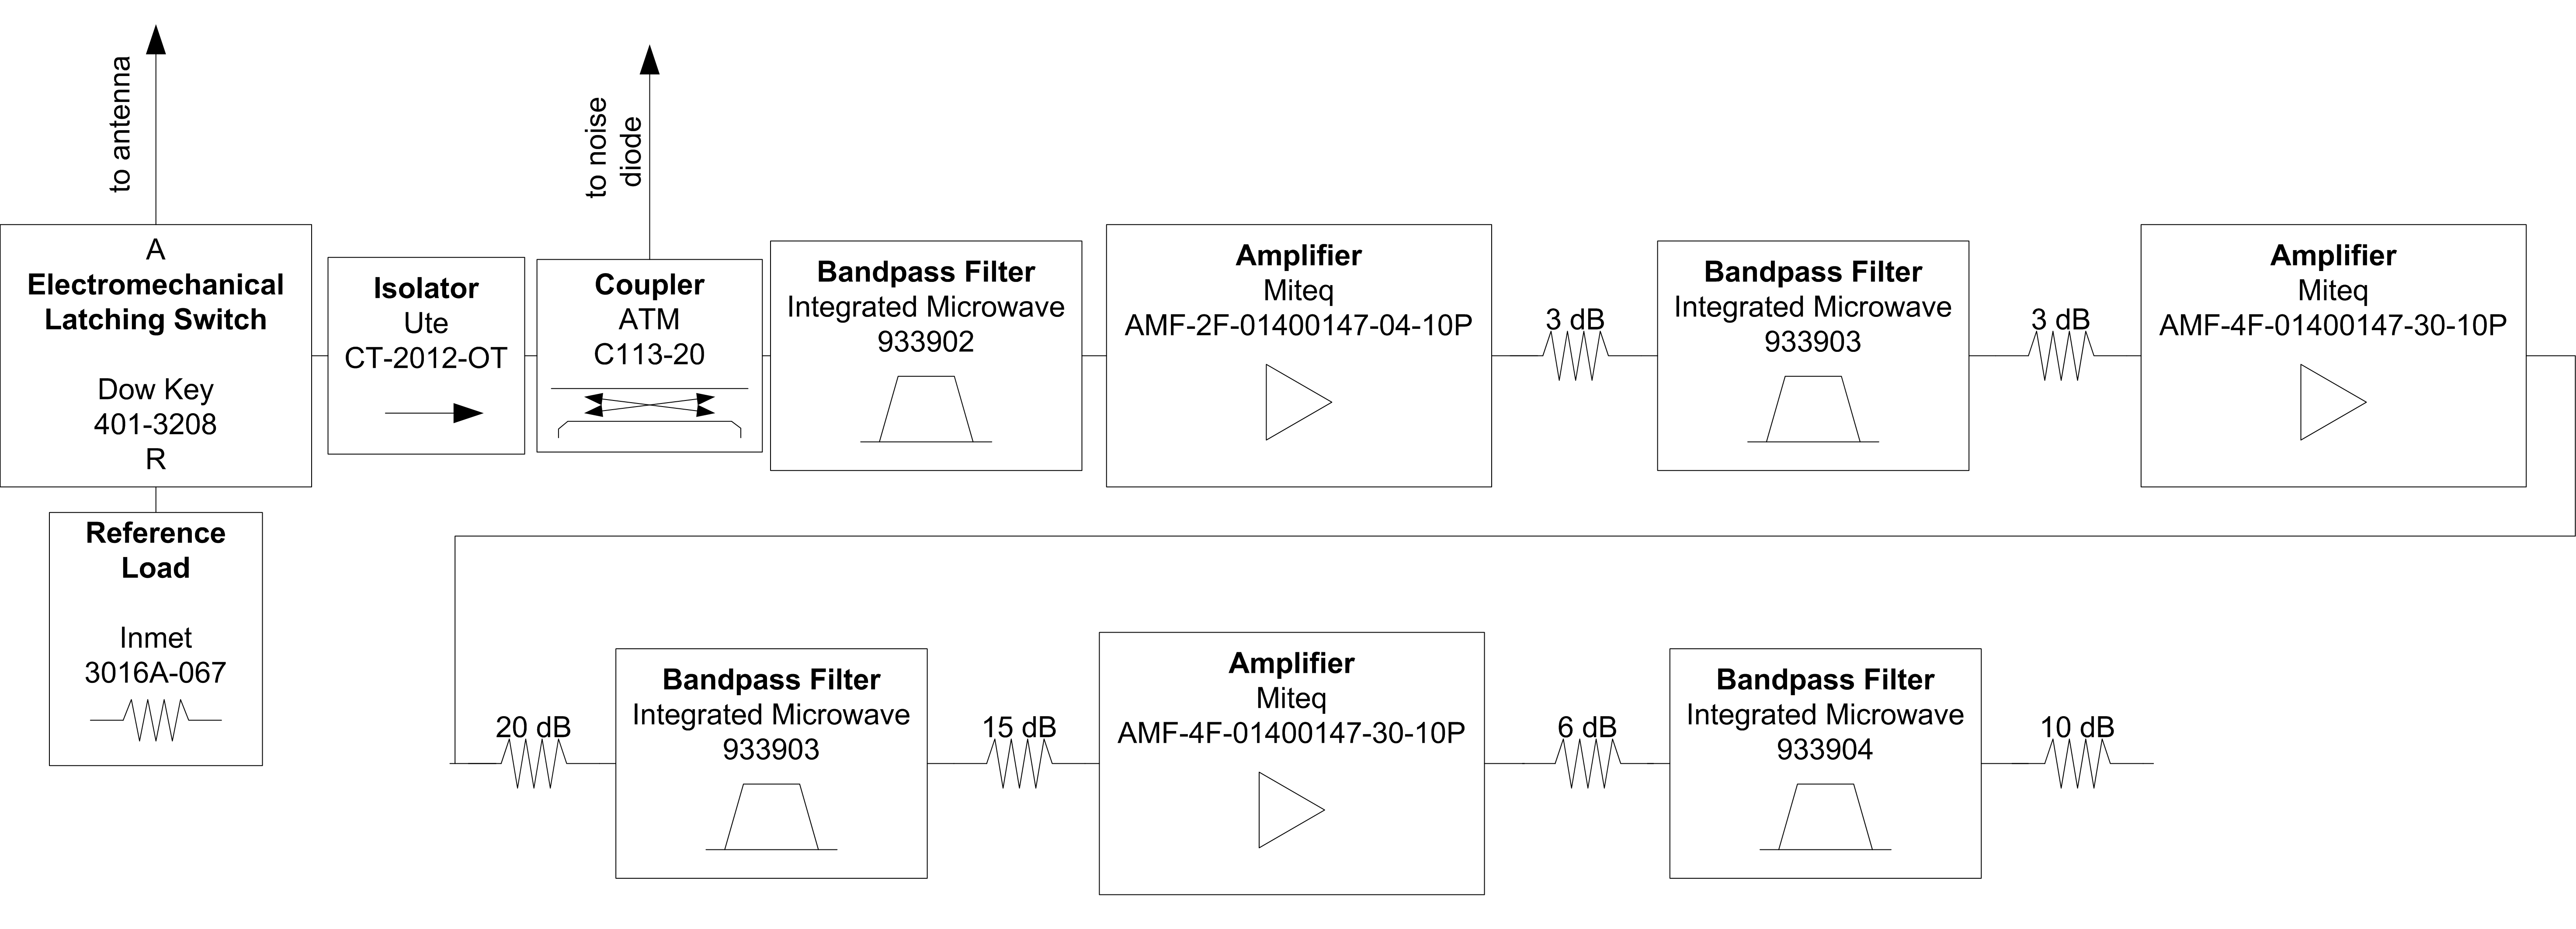
\includegraphics[width=17cm]{Images/ISU_rf_block.png}
%\isucaption{A block diagram provided by the University of Michigan that shows the components used in the ISU RF front end.}
%\label{ISU_rf_block}
%\end{figure}
%}

%As it can be seen in Figure \ref{ISU_rf_block} the current ISU rf front end uses a series of amplifiers, filters and attenuators to amplify and filter the incoming signals.  The attenuators are used to ensure that we do not overload the front end of the LNA proceeding it in the chain.  This RF chain provides us a spectrum from 1400 MHz to 1425 MHz and gives us a total gain of approximately 81 dBm.  This raises the noise floor to approximately -30 dBm which makes it very easy to detect with both a square-law detector and the software defined radio.  The performance of the ISU front end was confirmed by using a spectrum analyzer to look at the output signal and power output.  The spectrum analyzer output can be seen in Figure 

%{\begin{figure}[h!tb] 
%\centering
%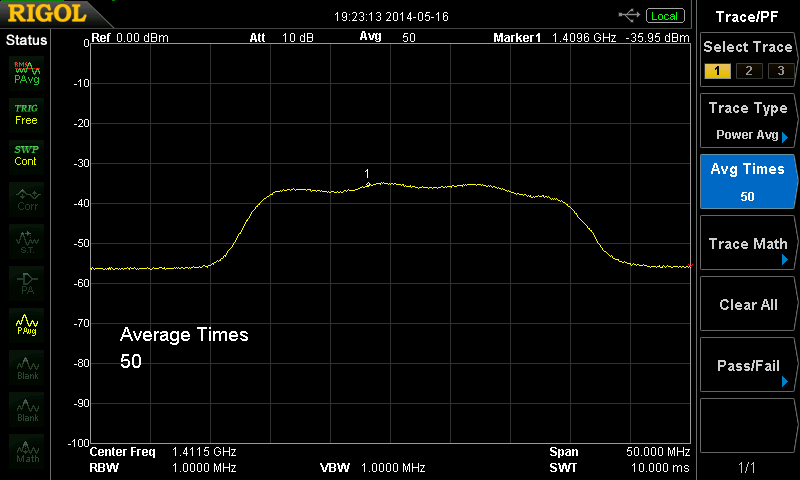
\includegraphics[width=17cm]{Images/radlidoff.png}
%\isucaption{A screenshot taken from a spectrum analyzer showing the filters and amplification done by the ISU Radio RF front end.}
%\label{ISU_rf_spectrum}
%\end{figure}
%}

%The ISU Radiometer front end was dismantled and was used for the experiments used in this thesis.  The LNAs and bandpass filters were kept intact to be used for experimentation.  While the bandpass filters were not needed for the software defined radio, since we were comparing our data to a square-law detector, they were still required for that device so that both the SDR and the Square-law detector could be looking at approximately the same signal.

%\subsubsection{A note about the ISU RF Front end}

%During the work on this thesis a few issues came up with the ISU RF front end that was used.  When work began on this thesis, it was assumed that the problems that were found with this hardware was limited to the digital portion of the radiometer.  This meant that the RF front end was performing as expected.  At first, early tests on the ISU RF front end seemed to confirm this as the output seen on a spectrum analyzer appeared to be normal.  However, further testing started to show unusual behavior.  Later, it was discovered that the ISU RF front end was prone to malfunctioning under certain conditions.  These conditions seemed to occur when the RF front end was moving on it's platform and even the lid to the box containing the RF front end would affect it.  

%A test was done to show this effect with the lid, and further information about the rotation affect is discussed in Appendix 2 in regards to the E E 518 laboratory experiment. For the lid experiment, a spectrum analyzer was hooked up to the ISU RF front end.  With the lid off, you can see what appears to be a normal signal that we would expect from the radiometer in Figure \ref{ISU_rf_spectrum}.  However, in Figure we placed the lid on the radiometer and the results are quite different.  Changes to the signal were observed in real time as the lid was placed on the radiometer and it was clear that this was also causing the radiometer to produce undesirable results.  

%{\begin{figure}[h!tb] 
%\centering
%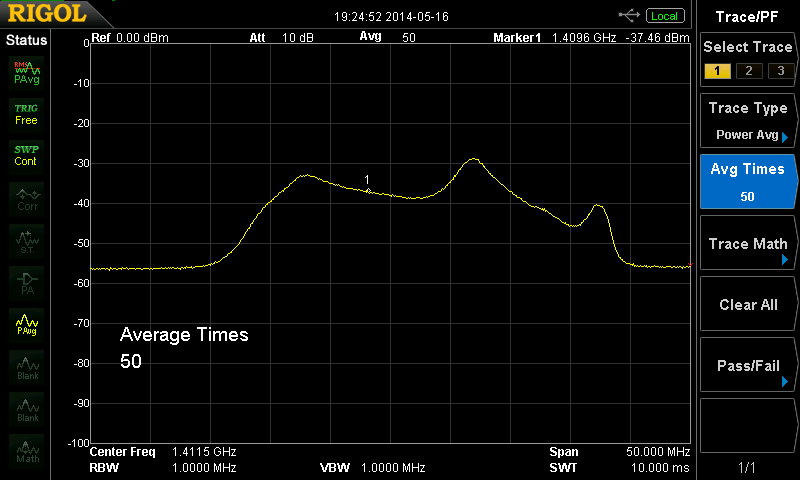
\includegraphics[width=17cm]{Images/lidpart.png}
%\isucaption{A screenshot taken from a spectrum analyzer showing the affect of the radiometers lid as it was placed on the radiometer.}
%\label{lid_on}
%\end{figure}
%}

%It was clear that there is something happening with the ISU RF front end.  This also points out another use for the addition of the software defined radio.  The old ISU radiometer system under-sampled the signal and so frequency information was lost.  Without hooking up something like a spectrum analyzer there would be no way for any to know what was happening with the ISU radiometer.  However, with the SDR we now have power and spectrum information.  In fact, it was during the E E 518 laboratory that we noticed a problem with the ISU radiometer and we discovered this by looking at the data that was captured by the SDR.  It was due to these issues that came up that the RF front end was rebuilt. 

%Work was done to re-stabilize and make the ISU radiometer front usable for the experiments used in this thesis.  First, all non-essential equipment was deactivated and powered down.  This included the on board microcontroler, the A/D converters and the FPGA unit that was originally used in this radiometer.  The thermal electric coolers were also deactivated as well.  Since the LNAs were in a temperature controlled room, they were not needed for these experiments.  

%Next, the LNAs were powered from a lab bench power supply instead of the power supplies that were used in the radiometer.  It is theorized that the power supplies feeding the radiometer may have been damaged due to water that had entered the case and were no longer stable in the power they provided.  To eliminate any issues, they were removed and a new and known to be working lab power supply was used to power both the LNAs and the square-law detector circuitry.   


